\section{Введение}
\label{sec:Chapter0} \index{Chapter0}

\subsection{Особенности задач машинного обучения}

За последние несколько лет методы машинного обучения (ML, от Machine Learning) продемонстрировали стремительный рост как в области применения, так и в качестве получаемых результатов.
В большинстве случаев этот прогресс стал возможен благодаря увеличению вычислительных мощностей используемых исполняющих сред.
Чтобы в полной мере оценить масштаб произошедших изменений, необходимо рассмотреть вычислительные требования, предъявляемые современными моделями, а также проанализировать особенности архитектур, на которых они исполняются.
Каждая программа исскустевнного интелекта (AI, от Artificial Intelligence) условно делится на два этапа: обучение и использование (инференс).
Этап обучения заключается в подаче большего количества разнообразных примеров, на основе которых модель адаптирует свои параметры, чтобы повысить способность к обобщению и точности предсказаний на новых, ранее не виденных данных.
Этот процесс достигается с помощью математических методов регрессии и оптимизации, таких как поиск локального минимума в многомерном параметрическом пространстве.
Целью является построение модели, приближённой к оптимальной для заданного распределения входных данных.
Характерной чертой большинства таких задач является возможность их формализации с использованием примитивов линейной алгебры.
В упрощённом виде модель можно представить как последовательность алгебраических операций над тензором параметров $X$ и входными данными $F$, где $F$ представляет собой пространство признаков, а $Y$ — соответствующее пространство ответов.
Результатом обучения является набор параметров (весов) $X$, таких, что выполняется следующее условие:

\begin{equation}
|XF - Y|_{\text{norm}} \rightarrow \min
\end{equation}

На этапе инференса модель применяется к новым данным. Это означает сохранение последовательности алгебраических операций (часто представляемых в виде графа) и загрузку ранее полученных значений параметров $X$ на конечное устройство.
В отличие от обучения, инференс не включает в себя процесс оптимизации — он лишь выполняет предсказание на основе уже обученных весов, что делает его значительно менее ресурсоёмким.
Тем не менее, в последние годы наблюдается постоянное увеличение размера моделей, выражающееся как в количестве параметров, так и в сложности вычислений.
Это ставит под вопрос возможность стабильной и быстрой работы моделей на конечных устройствах без потери качества или увеличения времени отклика.
На рисунке ниже представлена экспоненциальная тенденция роста количества операций при обучении современных моделей.
Этот рост напрямую коррелирует с вычислительной нагрузкой при их инференсе. Наблюдаемая зависимость в некотором смысле напоминает закон Мура, с той разницей, что вместо количества транзисторов речь идёт о росте размеров тензоров и значений их элементов.
Но за счёт чего физически компенсируется постоянно растущая сложность современных AI-моделей?

\begin{figure}[h]
\centering
\begin{overpic}[width=0.8\textwidth]{models_complexity.png}
\end{overpic}
\caption{Рост вычислительных требований при обучении современных моделей.}
\end{figure}

Вычислительно, процесс получения предсказания модели можно представить как последовательность вложенных циклов for, где каждая последующая строка соответствует проекции i-й координатной оси на итерационное пространство.
Конструкция вложенных циклов \texttt{for} представляет собой основную проблему при распараллеливании программ.
Это связано с множественными зависимостями данных, на основе которых можно построить \textbf{граф потока данных} (от англ. data flow graph).
Вершинами такого графа являются данные некоторой ячейки многомерного массива:

\[
A[i][j][k]\ldots[l][m]
\]

Ребро, проведённое из вершины \((a_1, b_1, c_1, d_1, \ldots)\) в вершину \((a_2, b_2, c_2, d_2, \ldots)\), обозначает необходимость значения первой ячейки для вычисления второй.
Обычно при построении графа потока данных выделяют следующие типы \textbf{зависимостей} данных:

\begin{enumerate}
    \item \textbf{Внутрициклические зависимости} - между итерациями одного цикла. Если текущая итерация зависит от предыдущей, это создает последовательную цепочку в графе.
    \item \textbf{Межциклические зависимости} - между разными уровнями вложенности. Внешний цикл может влиять на все итерации внутреннего цикла.
    \item \textbf{Диагональные зависимости} - когда элемент зависит от элементов на предыдущих итерациях обоих циклов одновременно.
\end{enumerate}

Data-flow граф широко применяется при разработке алгоритмов распараллеливания тензорных вычислений.
Тензорные вычисления являются основой современных программ искусственного интеллекта, что обусловливает необходимость их строгого и структурированного описания в рамках выполняемой задачи.
К числу типичных тензорных операций относятся, в частности, матричное умножение, свёртка тензоров, а также редукция по заданным осям тензорных структур.

Применение графа вычислительного потока при описании операций матричного умножения позволяет выявить повторяемость типов зависимостей между операциями и их регулярную структуру.
Так, каждый элемент результирующей матрицы $C[i][j]$ зависит от всех элементов $i$-й строки матрицы $A$ и $j$-го столбца матрицы $B$, что отражает характер тензорной зависимости и даёт основу для эффективного распараллеливания вычислений.

Подобная схема требует максимальной загрузки вычислительных ресурсов (CPU, GPU, NPU — подробнее о них ниже), что влечёт за собой значительные накладные расходы, включая потребление электроэнергии.
Вычислительные устройства можно условно расположить по шкале "приспособленности" к выполнению таких задач — от наименее до наиболее эффективных. Тогда иерархия будет выглядеть следующим образом:

$$CPU < GPU < NPU$$

Такое ранжирование обусловлено наличием аппаратной поддержки параллельных вычислений. Преимущество одного типа устройств над другим определяется степенью их специализации для конкретного класса задач.
Если отличия между CPU и GPU относительно хорошо понятны, то NPU (Neural Processing Unit, или ИИ-ускоритель, AI accelerator) представляет собой новый архитектурный подход к выполнению матричных операций.

В отличие от CPU и GPU, где требуется программная реализация эффективного параллелизма, NPU изначально сконструированы именно для этой задачи и реализуют регулярность зависимостей данных на уровне аппаратуры.
Примером такой микроархитектуры служит TPU (Google Tensor Processing Unit), в которой логические элементы располагаются так, что результат вычислений как бы «течёт» по микросхеме, распространяясь к её выходу.
Это обеспечивает аппаратный уровень конвейерной обработки и высокую степень параллелизма.

\begin{figure}[h]
\centering
\begin{overpic}[width=0.8\textwidth]{Google-TPU-micro.png}
\end{overpic}
\caption{Схема распространения вычислений в TPU.}
\end{figure}

В рамках данной работы различия в микроархитектуре перечисленных типов устройств не будут подробно рассматриваться.
Они приведены здесь лишь для иллюстрации того, как развивается аппаратная часть и какие решения предлагаются в ответ на растущие вычислительные требования современных моделей.
Важно подчеркнуть, что аппаратные средства активно эволюционируют, открывая всё больше возможностей для эффективного исполнения усложняющихся AI-моделей.

\subsection{Средства разработки ML-моделей}

Помимо аппаратных средств ускорения, существуют также программные подходы к оптимизации.

Основная сложность в данной области исследований заключается в разработке полноценной среды программирования и предоставлении библиотек, реализующих базовые математические абстракции.
Такие среды, или фреймворки, делают акцент на удобстве использования, простоте построения моделей, а также предоставлении инструментов для сжатия, профилирования и нативного исполнения моделей.

Появление этих фреймворков существенно упростило процесс разработки, снизив технический порог входа в область машинного обучения и способствовав стремительному росту объёма доступного кода.
В результате сформировалась масштабная кодовая база с широким спектром моделей, способных решать множество прикладных задач.

К наиболее популярным и широко применяемым фреймворкам сегодня относятся \textbf{TensorFlow}, \textbf{PyTorch} и \textbf{ONNX}.

Однако там, где достигается удобство, нередко приходится жертвовать производительностью — именно это изначально наблюдалось в перечисленных фреймворках.
Высокоуровневые математические конструкции, такие как тензорные операции, векторы, а также операции скалярного и векторного произведения, зачастую транслируются в исполняемый код довольно прямолинейно.
Под «прямолинейной» трансляцией подразумевается процесс, при котором тип и порядок высокоуровневых операций не учитываются при выборе возможных оптимизаций.
Оптимизации — такие как свёртка констант, планирование инструкций и машинно-зависимые преобразования — выполняются на уровне элементарных арифметических операций, что ограничивает общий прирост производительности.

\begin{figure}[h]
    \centering
    \begin{subfigure}{0.45\textwidth}
        \centering
        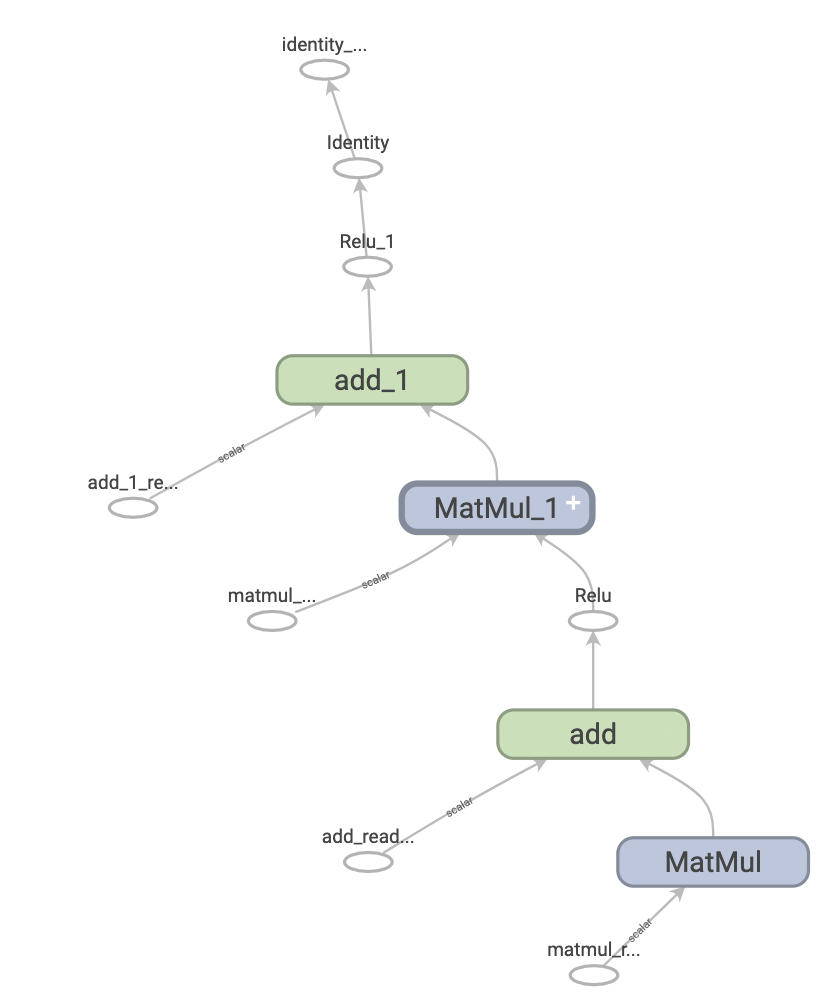
\includegraphics[width=\textwidth]{two-layer-network.png}
        \label{fig:sub2}
    \end{subfigure}
    \caption{Пример графа исполнения \textbf{Tensorflow}.}
    \label{fig:main}
\end{figure}

Становится очевидным, что разрыв между уровнями абстракции — от описания модели до низкоуровневой реализации — представляет собой незаполненную нишу, которую можно использовать для создания новых оптимизаций программ искусственного интелекта.

Одним из наиболее успешных и широко применяемых проектов в данной области является \textbf{ONNX Runtime} \cite{onnx_main}, разработанный компанией Microsoft.
Он предоставляет расширенные возможности для оптимизации и выполнения моделей, представленных в формате ONNX.
В рамках данного проекта было разработано собственное графовое промежуточное представление, на базе которого реализована многоуровневая система графовых оптимизаций.
Эта система позволяет эффективно преобразовывать вычислительные графы с целью повышения производительности и сокращения времени исполнения.

Процесс компиляции ONNX-моделей может быть схематично представлен в виде последовательности представлений:
\[\]
    \makebox[\linewidth]{ONNX $\rightarrow$ GraphIR $\rightarrow$ Execution Providers $\rightarrow$ Execution binary}
\[\]

Еще одиним удачным примером подобного подхода можно считать проект LLVM \cite{llvm_main}, получивший широкое распространение и продолжающий активно развиваться.
Ключевым преимуществом LLVM является высокая модульность и гибкость его архитектуры.
Это достигается благодаря введению промежуточного представления (англ. Intermediate Representation, IR), которое используется как основа для множества этапов компиляции и оптимизации.

\textbf{LLVM IR} \cite{llvm_main} сохраняет семантику исходной программы, написанной на высокоуровневом языке, но одновременно обладает структурой, близкой к ассемблерному коду.
Такое сочетание делает IR мощным инструментом для анализа и преобразования программ на этапе, независимом от целевой архитектуры.
Одним из главных достоинств LLVM IR является возможность реализации архитектурно-независимых оптимизаций, применяемых до генерации финального машинного кода. К таким оптимизациям можно отнести:

\begin{itemize}
    \item распространение констант (constant propagation),
    \item разворачивание циклов (loop unrolling),
    \item инлайнинг функций,
    \item переупорядочивание инструкций и устранение избыточных операций,
    \item \textbf{и многие другие.}
\end{itemize}

Важно отметить, что LLVM предоставляет расширяемую инфраструктуру, позволяя добавлять собственные типы, инструкции, метаинформацию и реализовывать пользовательские проходы оптимизации (passes).
Кроме того, LLVM IR активно используется в реализации оптимизаций, направляемых профилем выполнения (Profile-Guided Optimizations, PGO), где информация о поведении программы в реальных условиях позволяет проводить более эффективные преобразования.

Тем не менее, несмотря на выразительность и гибкость LLVM IR, он остается ориентированным на императивные языки общего назначения и ближе к низкоуровневой модели вычислений.
В условиях растущей сложности моделей машинного обучения, необходимости в высокоуровневых тензорных операциях, графовых представлениях и специфике разнообразных аппаратных ускорителей (GPU, NPU), возникает потребность в промежуточном представлении, способном отразить более абстрактные вычисления, сохраняя при этом поддержку всех преимуществ компиляторной инфраструктуры.

\subsection{Уровни абстракций и MLIR}

Именно по этой причине в апреле 2019 года был представлен новый проект от разработчиков LLVM, направленный на решение проблемы разрыва между уровнями абстракций в представлениях программ — MLIR.
\textbf{MLIR} (от англ. Multi-Level Intermediate Representation) \cite{mlir_main} представляет собой принципиально новый подход к описанию и трансформации высокоуровневых операций.
Само название — многоуровневое промежуточное представление — точно отражает основную идею проекта.
Используя модульную архитектуру LLVM, разработчики предложили расширяемую инфраструктуру, в рамках которой стало возможным создавать собственные уровни представления — так называемые диалекты (dialects).
Каждый диалект описывает специфический набор операций, типов и правил обработки, соответствующий определённому уровню абстракции.
Теперь, благодаря механизму lowering (понижение уровня представления), стало возможно последовательно преобразовывать программу с высокого уровня до низкоуровневого представления LLVM IR, контролируя и оптимизируя каждый этап компиляции.

Для современных фреймворков машинного обучения типичный процесс перехода по уровням абстракций выглядит следующим образом:
\begin{itemize}
    \item \textbf{TF} или \textbf{TFLite} - диалект уровня исходного кода моделей,
    \item \textbf{MHLO} или \textbf{TOSA} - диалект математических операций ML (присутствуют тензоры, батчи и др.),
    \item \textbf{LINALG} - диалект алгебры линейных операций (использует буферы вместо тензоров),
    \item \textbf{VECTOR} - диплект низкоуровневого векторного представления.
    \item \textbf{LLVM IR}
\end{itemize}


\begin{figure}[h]
\centering
\begin{overpic}[width=0.8\textwidth]{codegen-dialect-hierarchy.png}
\end{overpic}
\caption{Схема многоуровневого представления MLIR.}
\end{figure}

\textbf{Целью} данной работы является создание вспомогательного инструмента для \textbf{PGO} (Profile-Guided Optimization) в инфраструктуре MLIR на основе диалекта TensorFLow \cite{tf_mlir}, позволяющего проводить анализ участков исполнения программы, требующих непосредственной оптимизации.
Предлагается использовать существующие профилировщики программ машинного обучения и разработать расширение диалекта верхнего уровня за счёт добавления полей метаданных.
Такое отображение профиля исполнения на граф операций позволит принимать решения об оптимизации высокоуровневых операций на основе фактического поведения программы, при этом сохранив совместимость с широким набором существующих моделей.

\newpage
